\section{The CMS Computing Operations Workload}
\label{sec:workload}

CompOps operations cover three computing activities and pull
operator support from four information sources.
Section~\ref{sec:compops_domain} describes the activities and
the source layout; Section~\ref{sec:question_patterns}
introduces the 260-question evaluation set extracted from
production traffic; Section~\ref{sec:workflows} traces three
recurring workflows that exercise the tool families.

\subsection{Computing Operations at CMS}
\label{sec:compops_domain}

The three activities of Section~\ref{sec:introduction} (Tier-0,
P\&R, Data Management) all emit operational state into a shared
layer: workflow state, transfer rates, job-failure counts, and
site-readiness metrics are aggregated into MonIT and surfaced
through OpenSearch and Grafana~\cite{cms_monit}. CompOps
responsibilities split across operators, workflow managers, and
campaign managers, working in shifts across CERN, FNAL, INFN, and
other collaboration centres with daily handover on Mattermost and
ticket-driven escalation to on-call experts. Recurring questions in operator traffic include: where a
transfer is stuck, why a workflow has resubmitted five times,
which site is in downtime, what the runbook says about an error
code, whether a given Jira ticket is already known, and which
procedure a new team member should follow.

Four sources cover the answer space: the CMS TWiki holds the
documented procedures; the Jira project holds the ticket history
with assignees and resolutions; MonIT holds the time-series of
operational counters; and the \texttt{cms-comp-ops} Mattermost
channel holds the unwritten context not yet in a runbook.
Diagnosing a stalled transfer typically starts from the runbook
entry, requires the current MonIT counters and the site's
readiness status, and ends with the Jira-ticket history of past
stalls on that link.

\subsection{Operator Question Patterns}
\label{sec:question_patterns}

The 260-question evaluation set is sampled from the deployed
assistant's traffic between 16 February and 30 March 2026, after
deduplication and filtering of non-English messages, empty turns,
and development-team conversations; it exposes three patterns
relevant to the agent design.
First, operator questions split roughly evenly between
documentation and live state: 144 of 260 questions can be answered
from the documented procedure alone, and 116 require a live tool
call against Jira or MonIT.
Second, 108 of 260 questions (42\%) are part of a multi-turn
conversation: a follow-up such as ``which site was that?''
resolves only against the preceding turns.
Third, 55 of 260 questions (21\%) refer to time-sensitive
operational state, where an answer correct on Monday is wrong on
Friday.

We labelled each question with one of six categories chosen to
match how operators phrase their questions rather than how the
agent answers them.
The labels are assigned by a deterministic rule-based classifier
that walks each question through a fixed priority order: log-trace
dumps fall to \textit{debugging}; questions containing a CMS Jira
ticket reference (\texttt{CMSPROD-}, \texttt{CMSTRANSF-},
\texttt{CMSCOMPPR-}, $\dots$) fall to \textit{jira\_investigation};
questions about counts in a recent window fall to
\textit{data\_query}; imperative ``how do I'' patterns fall to
\textit{procedural}; ``summarize'' and ``explain'' patterns fall
to \textit{exploratory}; everything remaining is
\textit{factual\_lookup}.
We chose rule-based labelling over an LLM-assigned scheme because
the categories are defined by surface-form features and the
labelling has to be reproducible across curation passes.

The category distribution reflects the steady-state CompOps
workload during the six-week sampling window.
Factual lookups (76 questions, 29\%) are the largest single
category: examples include which storage element backs a given
site, what Rucio rule applies to a particular dataset, or what a
particular configuration value means.
Data queries (52 questions, 20\%) and Jira investigations (39
questions, 15\%) together account for the live-access half of the
workload: both require a tool call, but data queries hit MonIT
counters while Jira investigations hit the ticket history.
Procedural and exploratory questions (34 each, 13\%) follow.
Debugging questions (25, 10\%) are the smallest category and
cover cases where the operator dumps a full log into the chat.

The doc-answerable / live-access split follows the categories
deterministically: factual, procedural, and exploratory questions
are doc-answerable; data, Jira, and debugging questions require a
live tool call.
The agent has to handle both halves; the controls without
live-tool access (Section~\ref{sec:evaluation}) can only handle
the doc-answerable half by construction.
Figure~\ref{fig:workload} shows the breakdown.

\begin{figure}[htbp]
\centering
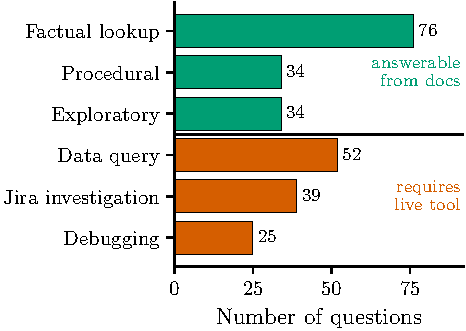
\includegraphics[width=\columnwidth]{figs/fig_workload.pdf}
\caption{Operator questions split roughly evenly between
documentation-answerable (144, green) and live-tool-required
(116, red) categories. The 260-question evaluation set by
category.}
\label{fig:workload}
\end{figure}

\subsection{Common operator workflows}
\label{sec:workflows}

Three workflows distilled from the recorded operator traffic
illustrate how the tool families combine.

\emph{Stalled transfer triage.} An operator sees a transfer to
a Tier-2 site failing and asks Archi why. The agent issues parallel
tool calls: an HTCondor MonIT aggregation over recent transfer
events, a CompOps Jira retrieval for tickets referencing the site
or source, and a CMS TWiki retrieval over the transfer-recovery
runbook. It returns the site-readiness status, the most recent
matching ticket, and the runbook section for the failure mode.

\emph{Workflow resubmission diagnosis.} For a workflow that has
resubmitted five times, the agent aggregates HTCondor MonIT
failure codes, retrieves the workflow's Jira ticket plus similar
past resubmissions, and looks up the resubmission runbook;
returns the failure pattern, prior resolutions, and recommended
action.

\emph{Procedure lookup.} For a stuck Tier-0 stream, the agent
retrieves the Tier-0 runbook from the TWiki and recent Tier-0
tickets from Jira; returns the recovery procedure and the most
recent tickets touching it.
